\documentclass[en]{subfiles}

\begin{document}

\section{Newton's Method}\label{sec:background_newton}

\subsection{Algorithm of Newton's Method}

In this subsection, we outline Newton's method, which is a fundamental optimization algorithm for an unconstrained optimization problem.
Newton's method is a representative iterative algorithm that starts from an initial point $x_0$, successively updates the current point, and generates a sequence $\{x_k\}_{k=0}^\infty$.

We assume that $f$ is of class $C^2$ and strongly convex, so that the Hessian matrix $\nabla^2 f(x)$ is positive definite for all $x \in \bbR^n$, and thus invertible.
Using the gradient $g_k \defeq \nabla f(x_k)$ and Hessian $\nabla^2 f(x_k)$ at the $k$-th iterate $x_k$, the base procedure of Newton's method is to iteratively update
\begin{equation*}
    x_{k+1} \gets x_k - \alpha_k \nabla^2 f(x_k)^{-1} g_k
\end{equation*}
with a step size $\alpha_k > 0$ determined by line search.
The derivation of this update rule is as follows.
The quadratic Taylor approximation of $f$ around $x_k$ is given by
\begin{equation}\label{eq:newton-model}
    m^*_{k}(x) \coloneqq f(x_k) + g_k^\top (x - x_k) + \frac{1}{2} (x - x_k)^\top \nabla^2 f(x_k) (x - x_k).
\end{equation}
The gradient of this model is
\begin{equation}\label{eq:newton-model-gradient}
    \nabla m^*_k(x) = g_k + \nabla^2 f(x_k)(x - x_k).
\end{equation}
Since the quadratic model \cref{eq:newton-model} is strongly convex by assumption, $x^* \in \bbR^n$ is the minimizer of $m^*_k$ if and only if $\nabla m^*_k(x) = 0$, so solving $\nabla^2 f(x_k)(x - x_k) = -g_k$ yields
\begin{equation*}
    \argmin_{x\in\bbR^n} m^*_{k}(x) = x_k -\nabla^2 f(x_k)^{-1} g_k.
\end{equation*}
Although this choice appears natural, it does not in general guarantee global convergence, as we will see in \cref{sec:newton-fullstep}.
Thus, we introduce a step size $\alpha_k > 0$ determined by line search to ensure a sufficient decrease in the function value.
This is the basic procedure of Newton's method.

The update direction $d_k \coloneqq -\nabla^2 f(x_k)^{-1} g_k$ is known as the Newton direction, which is a descent direction when the Hessian is positive definite, since
\begin{equation*}
    g_k^\top d_k = -g_k^\top \nabla^2 f(x_k)^{-1} g_k < 0.
\end{equation*}
If $f$ is nonconvex and the Hessian $\nabla^2 f(x_k)$ is negative definite or indefinite, function values are not guaranteed to decrease, and Newton's method may fail to converge.
Therefore, checking the positive definiteness of the Hessian is important when applying Newton's method.
The modified Newton method \citep[Sec. 3.4]{nocedal1999numerical} is one remedy for handling such cases.

\subsection{Properties Related to Convergence}
\label{sec:newton-local-convergence}

We next present a standard convergence theorem for Newton's method.

\subsubsection{Global Convergence}

We first state a general global convergence result
\begin{equation*}
    \lim_{k \to \infty} \norm{g_k} = 0
\end{equation*}
for methods with line search, and then explain its application to Newton's method.
We consider a general iterative method of the form
\begin{equation*}
    x_{k+1} \gets x_k + \alpha_k d_k,
\end{equation*}
where $d_k$ is a descent direction satisfying $g_k^\top d_k < 0$ and $\alpha_k > 0$ is the step size determined by line search.
We employ the Wolfe conditions \citep[Sec. 3.1]{nocedal1999numerical} to determine the step size $\alpha_k$ as follows:
\begin{align}
    f(x_k + \alpha_k d_k) & \leq f(x_k) + c_1 \alpha_k g_k^\top d_k, \label{eq:wolfe-1} \\
    g_{k+1}^\top d_k      & \geq c_2 g_k^\top d_k, \label{eq:wolfe-2}
\end{align}
where $0 < c_1 < c_2 < 1$ are constants.
We also define the angle between the direction $d_k$ and the negative gradient $-g_k$ as
\begin{equation}\label{eq:angle-definition}
    \cos \theta_k \coloneqq \frac{-g_k^\top d_k}{\norm{g_k}\norm{d_k}}.
\end{equation}
The following theorem is a simplified version of the classical result.

\begin{theorem}[{\cite[Theorem 3.2]{nocedal1999numerical}}]
    \label{thm:line-search-global-convergence}
    Suppose that $f$ is of class $C^1$ and bounded below in $\bbR^n$, and $L$-smooth.
    Consider the iterative method defined by
    \begin{equation*}
        x_{k+1} \gets x_k + \alpha_k d_k,
    \end{equation*}
    starting from an initial point $x_0 \in \bbR^n$, and the step size $\alpha_k$ is determined by the Wolfe conditions \cref{eq:wolfe-1,eq:wolfe-2}.
    For the angle $\theta_k$ defined in \cref{eq:angle-definition}, if there exists a positive constant $\delta$ such that
    $\cos \theta_k \geq \delta > 0$ for all $k$,
    then, the method generates a sequence $\{x_k\}$ satisfying
    \begin{equation}\label{eq:gradient-convergence}
        \lim_{k \to \infty} \norm{g_k} = 0.
    \end{equation}
\end{theorem}
\begin{proof}
    From the Wolfe condition \eqref{eq:wolfe-2}, we have
    \begin{equation*}
        (g_{k+1} - g_k)^\top d_k
        = g_{k+1}^\top d_k - g_k^\top d_k
        \geq (c_2 - 1) g_k^\top d_k,
    \end{equation*}
    and
    \begin{align*}
        (g_{k+1} - g_k)^\top d_k        & \leq
        \norm{g_{k+1} - g_k} \norm{d_k} &                                        & \text{(Cauchy--Schwarz inequality)}                           \\
                                        & \leq L \norm{x_{k+1} - x_k} \norm{d_k} &                                     & \text{($L$-smoothness)} \\
                                        & = \alpha_k L \norm{d_k}^2.
    \end{align*}
    By combining these two relations, we obtain
    \begin{equation}\label{eq:step-size-lower-bound-in-Wolfe}
        \alpha_k \geq \frac{c_2 - 1}{L} \frac{g_k^\top d_k}{\norm{d_k}^2}.
    \end{equation}
    and thus
    \begin{align*}
        f(x_{k+1}) & \leq f(x_k) + c_1 \alpha_k g_k^\top d_k                                   &  & \text{(Wolfe condition \eqref{eq:wolfe-1})}           \\
                   & \leq f(x_k) - c_1 \frac{1 - c_2}{L} \frac{(g_k^\top d_k)^2}{\norm{d_k}^2} &  & \text{(by \eqref{eq:step-size-lower-bound-in-Wolfe})} \\
                   & = f(x_k) - c_1 \frac{1 - c_2}{L} \cos^2 \theta_k \norm{g_k}^2.            &  & \text{(definition in \eqref{eq:angle-definition})}
    \end{align*}
    By summing this expression over all indices less than or equal to $k$, we obtain
    \begin{equation}\label{eq:telescoping-sum-Wolfe}
        f(x_{k+1}) \leq f(x_0) - c_1 \frac{1 - c_2}{L} \sum_{j=0}^k \cos^2 \theta_j \norm{g_j}^2.
    \end{equation}
    Since $f$ is bounded below, we have that $f(x_0) - f(x_{k+1})$ is less than some positive constant for all $k$.
    Hence, by taking limits in \eqref{eq:telescoping-sum-Wolfe}, we obtain the Zoutendijk condition:
    \begin{equation}\label{eq:zoutendijk}
        \sum_{k=0}^\infty \cos^2 \theta_k \norm{g_k}^2 < \infty.
    \end{equation}
    This condition implies that
    \begin{equation*}
        \cos^2 \theta_k \norm{g_k}^2 \to 0.
    \end{equation*}
    Combined with the assumption that $\cos \theta_k \geq \delta > 0$ for all $k$, it follows immediately that
    \begin{equation*}
        \lim_{k \to \infty} \norm{g_k} = 0,
    \end{equation*}
    which completes the proof.
\end{proof}

Since Newton's method is a special case of the setting in \cref{thm:line-search-global-convergence} with $d_k = -\nabla^2 f(x_k)^{-1} g_k$, we can apply this result under appropriate conditions of $f$.
In particular, if $f$ is $L$-smooth and $\mu$-strongly convex, then for any $k$, we have
\begin{equation*}
    \cos \theta_k
    = \frac{g_k^\top \nabla^2 f(x_k)^{-1} g_k}{\norm{g_k}\norm{\nabla^2 f(x_k)^{-1} g_k}}
    \geq \frac{\norm{g_k}^2 \lambda_{\min}(\nabla^2 f(x_k)^{-1})}{\norm{g_k}^2 \lambda_{\max}(\nabla^2 f(x_k)^{-1})}
    \geq \frac{\mu}{L},
\end{equation*}
where $\lambda_{\min}(\cdot)$ and $\lambda_{\max}(\cdot)$ denote the minimum and maximum eigenvalues, respectively.
Thus, by setting $\delta = \mu / L$ in \cref{thm:line-search-global-convergence}, we obtain the global convergence of Newton's method for strongly convex and smooth functions under line search satisfying the Wolfe conditions.

\subsubsection{Local Quadratic Convergence}

We next present a classical result on the local convergence rate of Newton's method.
We again provide a simplified version for brevity as follows.

\begin{theorem}[{\cite[Theorem 3.5]{nocedal1999numerical}}]
    \label{thm:newton-quadratic}
    Suppose that the Hessian matrix $\nabla^2 f(x)$ is Lipschitz continuous in a neighborhood of the solution $x^*$, and that sufficient second-order optimality conditions hold (i.e., $\nabla f(x^*)=0$ and $\nabla^2 f(x^*)$ is positive definite).
    If $\alpha_k=1$ for all $k$ and the initial point $x_0$ is sufficiently close to $x^*$,
    then the sequence of gradient norms $\{\norm{\nabla f(x_k)}\}$ converges quadratically.
\end{theorem}
\begin{proof}
    From the definition of the Newton step and the optimality condition $\nabla f(x^*)=0$, we obtain
    \begin{align*}
        x_{k+1} - x^*
         & = x_k - x^* - \qty(\nabla^2 f(x_k))^{-1}\nabla f(x_k)                                          \\
         & = \qty(\nabla^2 f(x_k))^{-1} \qty(\nabla^2 f(x_k)(x_k-x^*)-\qty(\nabla f(x_k)-\nabla f(x^*))).
    \end{align*}
    By Taylor's theorem and the triangle inequality, we have
    \begin{align*}
                & \norm{\nabla^2 f(x_k)(x_k-x^*)-\qty(\nabla f(x_k)-\nabla f(x^*))}                     \\
        =   {}  & \norm{\nabla^2 f(x_k)(x_k-x^*)-\int_0^1 \nabla^2 f(x_k+t(x^*-x_k)) (x_k - x^*)\dd{t}} \\
        \leq {} & \int_0^1 \norm{\nabla^2 f(x_k)-\nabla^2 f(x_k+t(x^*-x_k))}\norm{x_k-x^*}\dd t.
    \end{align*}
    If $\nabla^2 f$ is Lipschitz continuous with constant $L^{\mathrm{H}}$, then the integrand is bounded by $L^{\mathrm{H}}t\norm{x_k-x^*}$, and integrating yields
    \begin{equation*}
        \norm{\nabla^2 f(x_k)(x_k-x^*)-\qty(\nabla f(x_k)-\nabla f(x^*))}
        \le \frac{1}{2}L^{\mathrm{H}}\norm{x_k-x^*}^2.
    \end{equation*}

    Since $\nabla^2 f(x^*)$ is non-singular, there exists a radius $r>0$ such that for all $x_k$ satisfying $\norm{x_k-x^*}\le r$,
    \[
        \norm{\qty(\nabla^2 f(x_k))^{-1}}\le 2\norm{\qty(\nabla^2 f(x^*))^{-1}}
    \]
    holds.
    Combining these results, we obtain
    \begin{equation*}
        \norm{x_{k+1} - x^*}
        \le L^{\mathrm{H}}\norm{\qty(\nabla^2 f(x^*))^{-1}} \norm{x_k-x^*}^2.
    \end{equation*}
    Let $\widetilde L  \defeq  L^{\mathrm{H}}\norm{\qty(\nabla^2 f(x^*))^{-1}}$.
    If the initial point is chosen such that $\norm{x_0-x^*}\le \min\{r,1/(2\widetilde L)\}$, then by induction $\{x_k\}$ remains within the neighborhood and converges to $x^*$.
    The above error bound implies quadratic convergence of $\{x_k\}$.

    To show quadratic convergence of the gradient norm, we use $x_{k+1}-x_k=-\qty(\nabla^2 f(x_k))^{-1}\nabla f(x_k)$ and
    $\nabla f(x_k)+\nabla^2 f(x_k)\qty(x_{k+1}-x_k)=0$, yielding
    \begin{align*}
        \norm{\nabla f(x_{k+1})}
         & = \norm{\nabla f(x_{k+1})-\nabla f(x_k)-\nabla^2 f(x_k)\qty(x_{k+1}-x_k)}                  \\
         & \le \int_0^1 \norm{\nabla^2 f(x_k+t (x_{k+1}-x_k))-\nabla^2 f(x_k)}\norm{x_{k+1}-x_k}\dd t \\
         & \le \frac{1}{2}L^{\mathrm{H}}\norm{x_{k+1}-x_k}^2                                          \\
         & \le \frac{1}{2}L^{\mathrm{H}}\norm{\qty(\nabla^2 f(x_k))^{-1}}^2\norm{\nabla f(x_k)}^2     \\
         & \le 2 L^{\mathrm{H}} \norm{\qty(\nabla^2 f(x^*))^{-1}}^2\norm{\nabla f(x_k)}^2.
    \end{align*}
    Therefore, $\norm{\nabla f(x_k)}$ converges quadratically to zero.
\end{proof}

These propositions \cref{thm:line-search-global-convergence,thm:newton-quadratic} indicate that Newton's method equipped with line search has both global convergence and local quadratic convergence properties under appropriate conditions.
This rapid convergence is a significant advantage of Newton's method compared to first-order methods such as gradient descent, which typically exhibit only linear convergence.
However, computing the Hessian $\nabla^2 f(x_k) \in \bbR^{n \times n}$ and solving the linear system $\nabla^2 f(x_k) d_k = -\nabla f(x_k)$ require $\order{n^3}$ time, which is prohibitively expensive for large-scale problems.
Other optimization methods, such as quasi-Newton methods, are also used for such methods, as we will discuss later.

\subsection{Elements for Global Convergence}

As mentioned earlier, the positive definiteness of the Hessian matrix and the selection of the step size via line search play important roles in Newton's method.
In this subsection, we explain why these elements are required.

\subsubsection{Positive Definiteness of the Hessian Matrix}

We have assumed that $f$ is strongly convex so far, meaning that the Hessian matrix $\nabla^2 f(x_k)$ is positive definite at each iteration.
This assumption is crucial for Newton's method to converge locally to an optimal solution.
When the Hessian matrix is positive definite, Newton's method provides a descent direction toward the optimal solution, since
\begin{equation*}
    \nabla f(x_k)^\top d_k
    = -\nabla f(x_k)^\top \qty(\nabla^2 f(x_k))^{-1} \nabla f(x_k)
    < 0.
\end{equation*}
In contrast, when the Hessian matrix is negative definite or indefinite, a decrease in the function value is not guaranteed, and Newton's method may point in a direction that moves away from the optimal solution.
In the indefinite case, the function value may decrease, but the risk of converging to a saddle point is also increased.
Therefore, verifying the positive definiteness of the Hessian matrix is an important consideration when applying Newton's method.


\subsubsection{Issues with Full Steps}
\label{sec:newton-fullstep}

In Newton's method, adopting a step size $\alpha_k=1$ at every iteration may lead to difficulties.
Here, we present examples illustrating this issue and discuss the necessity of line search as a remedy.

\paragraph{An Example Where Newton's Method Diverges}

Consider the following function:
\begin{align*}
    f(x)   & = \sqrt{1 + x^2},            \\
    f'(x)  & = \frac{x}{\sqrt{1 + x^2}},  \\
    f''(x) & = \frac{1}{(1 + x^2)^{3/2}}.
\end{align*}
When the absolute value of the initial point exceeds 1, Newton's method diverges, as shown in \cref{fig:newton_failure_sqrt_function}.

\begin{figure}[t]
    \centering
    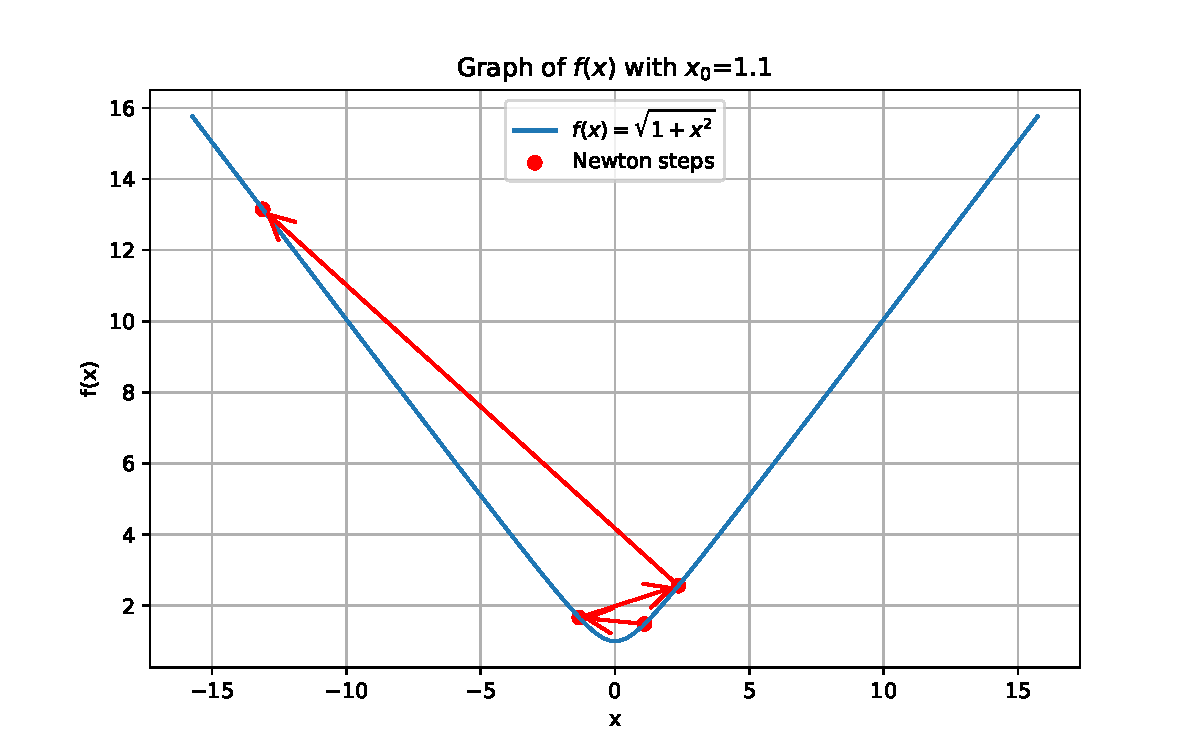
\includegraphics[width=0.6\textwidth]{../imgs/quasi_newton/newton_failure_sqrt_function_1.1.pdf}
    \caption{An example where Newton's method diverges with initial point $x_0=1.1$}
    \label{fig:newton_failure_sqrt_function}
\end{figure}

\paragraph{Oscillation of Newton's Method for Strongly Convex Functions}

In the previous example, the objective function was not strongly convex and did not necessarily possess favorable properties.
However, even for functions with the strong convexity property, there exist examples where Newton's method fails to converge \citep[Example 1.4.3]{Doikov2021SecondOrderTensor}.

In this example, for $\mu>0$, consider the function
\begin{align*}
    f(x)     & = \log(1 + e^x) - \frac{x}{2} + \frac{\mu x^2}{2}, \\
    f'(x)    & = \frac{e^x}{1+e^x} - \frac{1}{2} + \mu x,         \\
    f''(x)   & = \frac{e^x}{(1+e^x)^2} + \mu,                     \\
    f'''(x)  & = \frac{e^x(1 - e^x)}{(1+e^x)^3},                  \\
    f''''(x) & = \frac{e^x(1 - 4e^x + e^{2x})}{(1+e^x)^4}.
\end{align*}

This function has the following properties:
\begin{enumerate}[nosep,label=\textbullet]
    \item It is $\mu$-strongly convex.
    \item $\max_x |f''(x)| = \frac{1}{4} + \mu$ (attained at $e^x=1$). Hence, $\nabla f$ is $L$-smooth with $L=\frac{1}{4}+\mu$.
    \item $\max_x |f'''(x)| = \frac{1}{6\sqrt{3}}$ (attained at $e^x=2-\sqrt{3}$). Hence, $\nabla^2 f$ is $M$-Lipschitz with $M=\frac{1}{6\sqrt{3}}$.
\end{enumerate}

Nevertheless, when the initial point $x_0$ is sufficiently large relative to $\mu$, Newton's method exhibits oscillatory behavior, as shown in \cref{fig:newton_failure_strongly_convex_function}.

\begin{figure}[t]
    \begin{minipage}{0.5\textwidth}
        \centering
        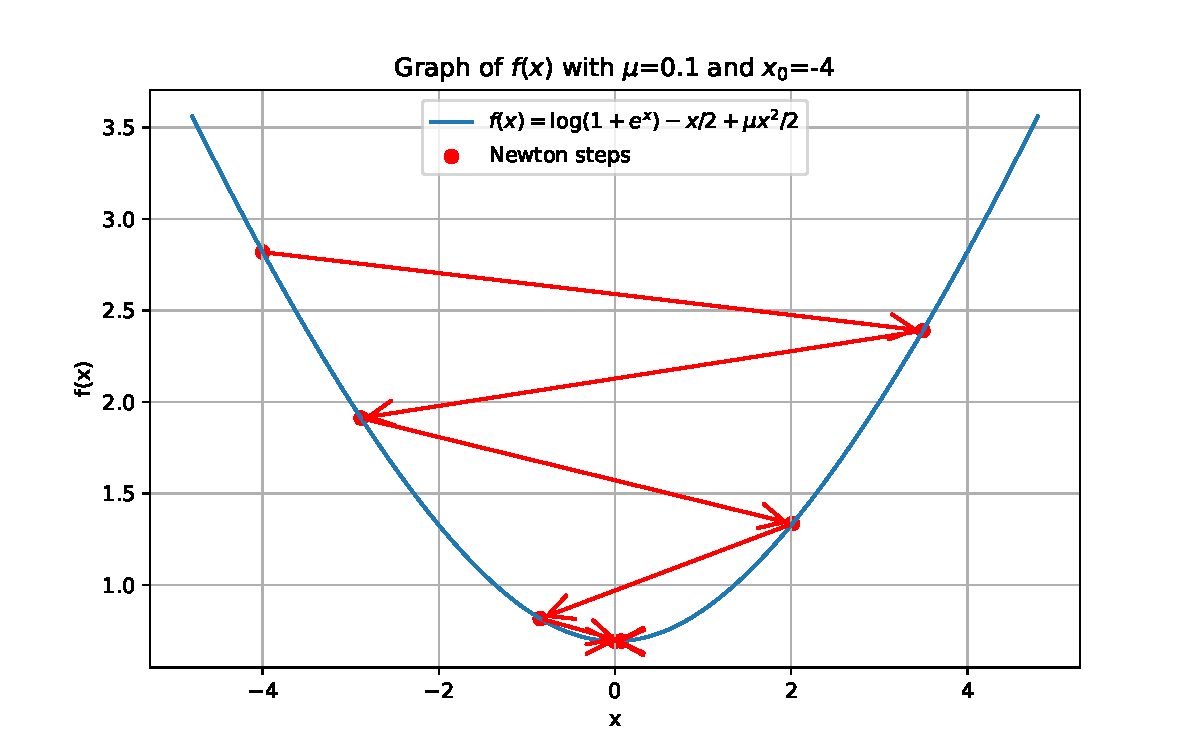
\includegraphics[width=\textwidth]{../imgs/quasi_newton/newton_failure_strongly_convex_function_0.1_-4.pdf}
    \end{minipage}%
    \begin{minipage}{0.5\textwidth}
        \centering
        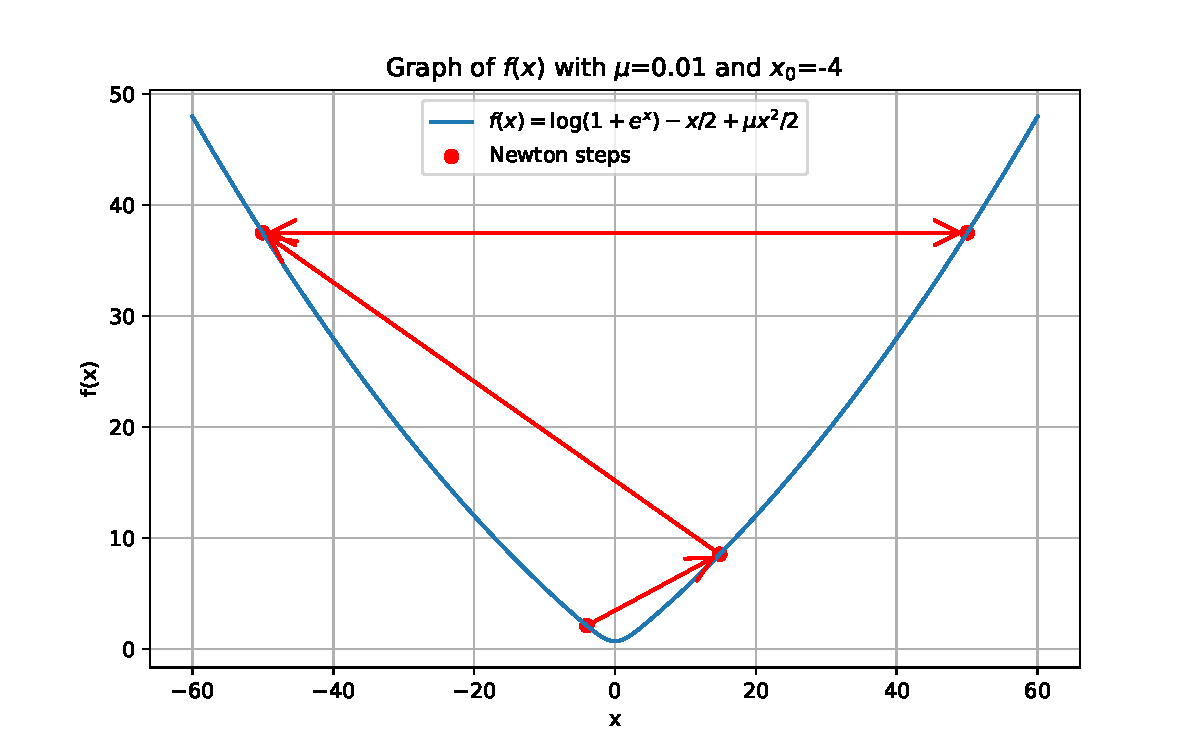
\includegraphics[width=\textwidth]{../imgs/quasi_newton/newton_failure_strongly_convex_function_0.01_-4.pdf}
    \end{minipage}
    \caption{(Left) Newton's method converges for $x_0=-4, \ \mu=0.1$; (Right) Newton's method oscillates for $x_0=-4, \ \mu=0.01$}
    \label{fig:newton_failure_strongly_convex_function}
\end{figure}

\paragraph{Necessity of Line Search}

To avoid the issues described above, it is common practice to select the step size $\alpha_k$ appropriately using a line search.
Newton's method equipped with line search is often referred to as the modified Newton method and is known to possess global convergence properties.

\subsection{Comparison with Newton's Method as a Root-Finding Algorithm}

As a conceptual supplement, we briefly clarify the relationship between ``Newton's method as a root-finding algorithm'' and ``Newton's method in optimization.''
These two formulations are closely related, but they have different perspectives and applications.

\subsubsection{Newton's Method as a Root-Finding Algorithm}

When referring simply to Newton's method (or the Newton--Raphson method), one often means a root-finding algorithm for a differentiable scalar function $g\colon \mathbb{R} \to \mathbb{R}$ that solves $g(x) = 0$.
Although this is not the main topic of this section, it is arguably more fundamental and widely known.

Starting from an initial value $x_0$, the iteration is given by
\begin{equation*}
    x_{k+1} = x_k - \frac{g(x_k)}{g'(x_k)}.
\end{equation*}
Geometrically, this corresponds to approximating the graph of $g$ near $x_k$ by its tangent line and selecting the intersection of this tangent with the $x$-axis as the next approximate solution.

\subsubsection{Newton's Method in Optimization}

In the context of optimization, Newton's method typically refers to an algorithm for finding a local minimizer of a twice-differentiable function $f\colon \mathbb R^{n} \to\mathbb{R}$, or equivalently, a stationary point satisfying $\nabla f(x) = 0$ as a necessary condition.
This is the primary focus of the present section.

Recall the assumption that the Hessian matrix $\nabla^2 f(x)$ is positive definite at each iteration.
Newton's method in optimization applies the framework of the root-finding algorithm to the gradient $\nabla f(x)$:
\begin{equation*}
    x_{k+1} = x_k - \nabla^2 f(x_k)^{-1} \nabla f(x_k).
\end{equation*}
In the scalar case, this reduces to $x_{k+1}=x_k - f'(x_k) / f''(x_k)$.

\subsubsection{Relationship Between the Two Formulations}

\begin{figure}[t]
    \centering
    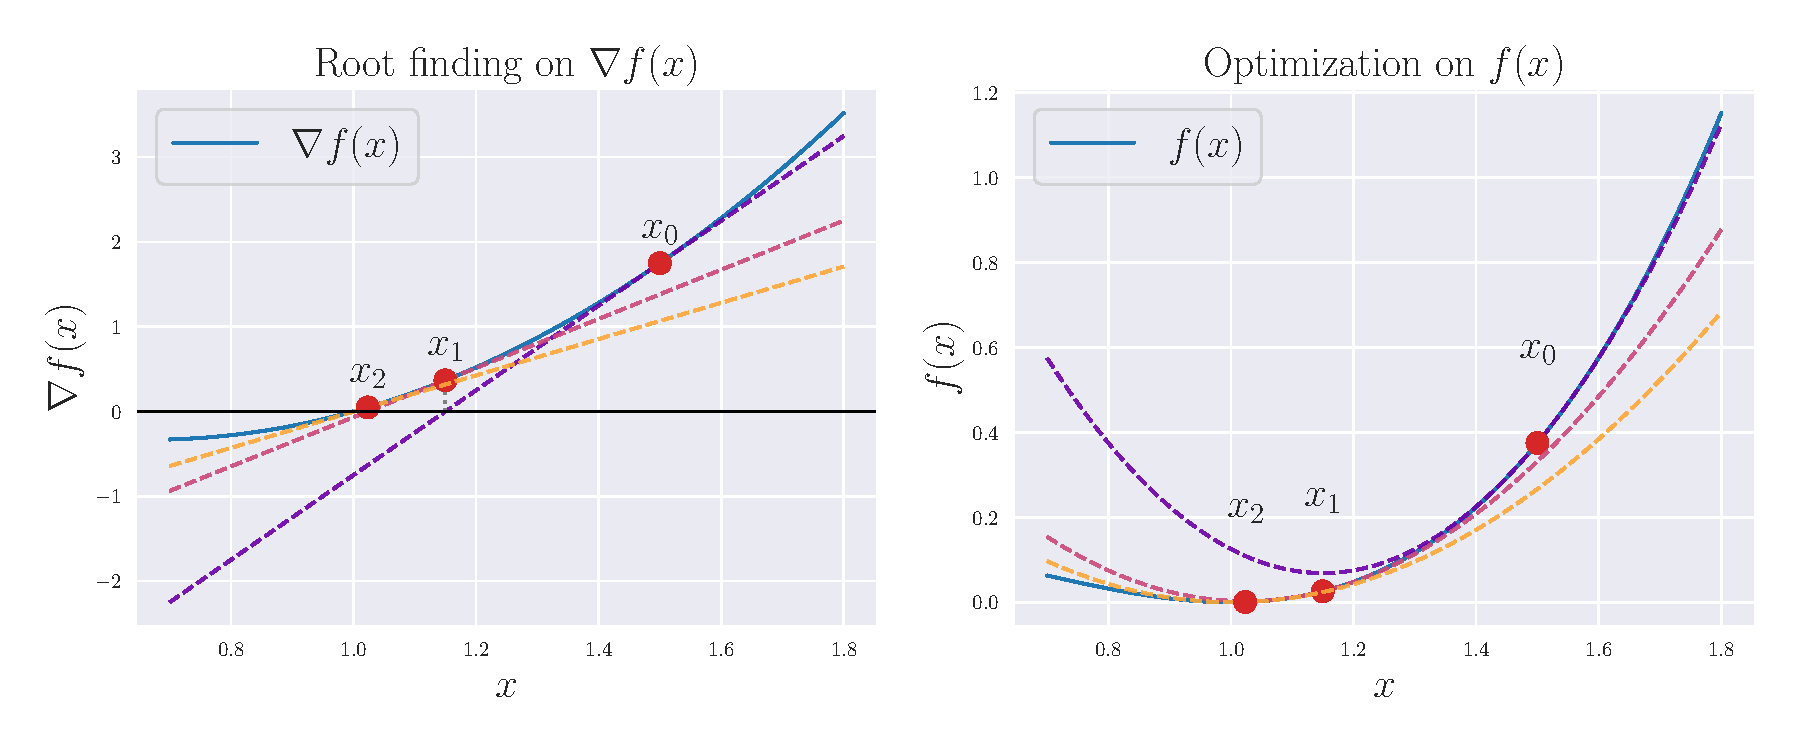
\includegraphics[width=\textwidth]{../imgs/quasi_newton/newton_raphson.pdf}
    \caption{Root-finding for the gradient $\nabla f(x)=3 x^2 - 4 x + 1$ and optimization of the function $f(x)=x^3 - 2 x^2 + x$}
    \label{fig:newton_raphson}
\end{figure}

Let us examine the equivalence of the two formulations through a concrete example.
\Cref{fig:newton_raphson} illustrates the relationship between these formulations using a simple cubic function $f(x)$.
The left panel shows root-finding applied to $g(x) = \nabla f(x)$, while the right panel shows optimization applied to $f(x)$.

In the root-finding formulation, $\nabla f(x) = 3x^2 - 4x + 1$ is approximated by its tangent line, namely
\begin{equation*}
    \nabla m^*_k(x) = \nabla f(x_k) + \nabla^2 f(x_k)(x - x_k),
\end{equation*}
and the root of this linear model is chosen as $x_{k+1}$.

In contrast, in the optimization formulation, $f(x) = x^3 - 2x^2 + x$ is approximated by its second-order Taylor expansion
\begin{equation*}
    m^*_k(x) = f(x_k) + \nabla f(x_k)(x - x_k) + \frac{1}{2}\nabla^2 f(x_k)(x - x_k)^2,
\end{equation*}
and the minimizer of this quadratic model is taken as $x_{k+1}$.

Thus, under the assumption of positive definiteness, it is clear from the properties of local solutions that both formulations perform essentially equivalent operations, and their correspondence can be explicitly verified.

In what follows, we consider only the optimization formulation.

\ifSubfilesClassLoaded{
    \bibliographystyle{plainnat}
    \bibliography{../L-BFGS.bib}
}{}

\end{document}
